\section{Final Implementation}

%----------------------------------------------------------------------------------------
%	Subsection
%----------------------------------------------------------------------------------------

\begin{frame}
\frametitle{Final Implementation}

\begin{enumerate}
	\item Coefficients that intensively require floating-point computations are precomputed.
	\begin{itemize}
		\item Hamming window, Mel-bank filter gain, discrete cosine transform
	\end{itemize}
\end{enumerate}

\begin{itemize}
\item Hamming window:
\begin{equation}
1 - \frac{0.014552 \text{ ms}}{1.012452 \text{ ms}} = 99\%
\end{equation}
\item DCT:
\begin{equation}
1 - \frac{0.006482 \text{ ms}}{0.287135 \text{ ms}} = 98\%
\end{equation}
\end{itemize}
\end{frame}

\begin{frame}
\begin{enumerate}
	\setcounter{enumi}{1}
	\item Special data structures are designed for sparse matrices.
	\begin{itemize}
		\item Mel bank filter gain, inversed variance matrices, transition matrices
		\item Meaningless multiplications with zeros are illuminated.
	\end{itemize}
\end{enumerate}

\begin{figure}[H]
\centering
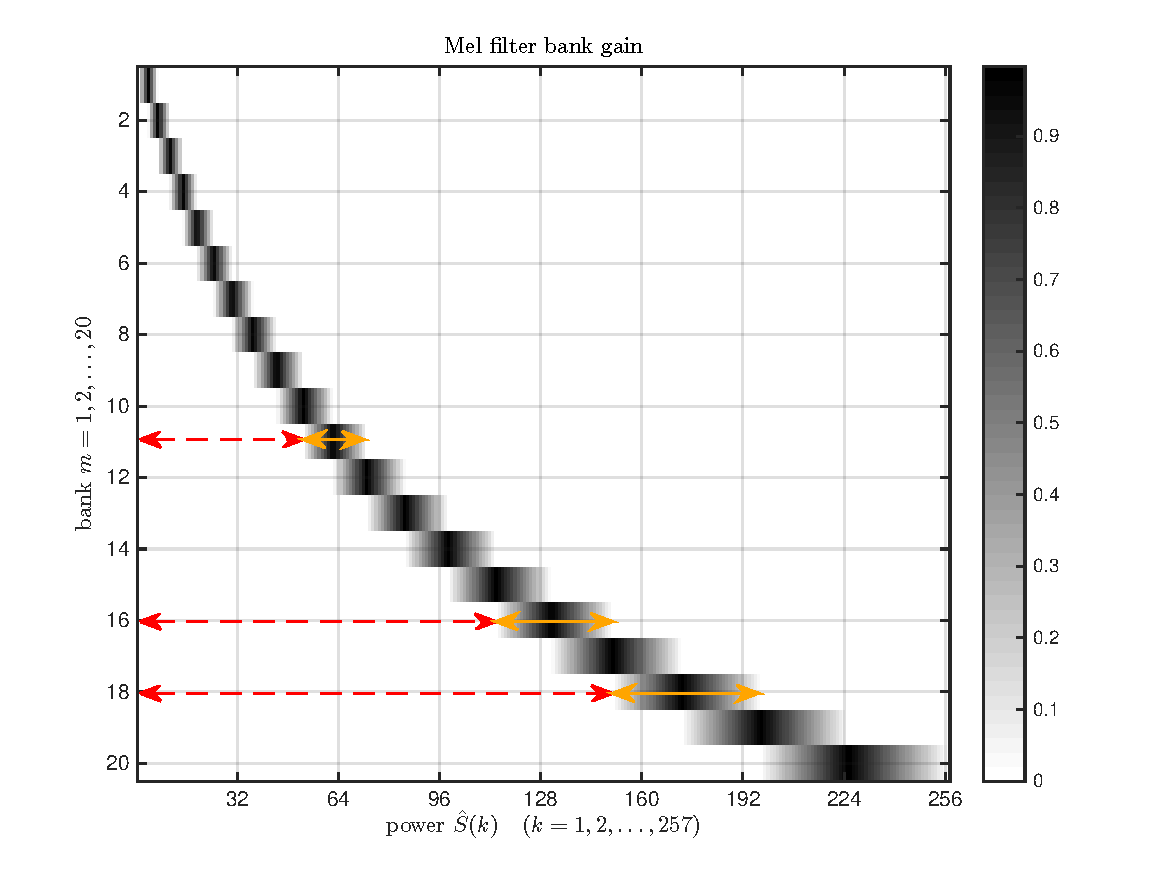
\includegraphics[width=3in, trim={0 0.6cm 0 0.6cm}, clip]{ang/mel_filter_bank_gain}
\caption{Mel filter bank gain}
\end{figure}
\end{frame}

\begin{frame}
\begin{enumerate}
	\setcounter{enumi}{2}
	\item Symmetry is sufficiently taken in to consideration.
	\begin{itemize}
		\item FFT of real sequence, discrete cosine transform
	\end{itemize}
\end{enumerate}

\begin{equation}
S_j[k] = \sum_{n=1}^{N} s_j[n] W_N^{(n-1) k} \quad k = 1, 2, \dots, N
\end{equation}
\begin{equation}
\hat{S}_j[k] = |S_j[k]|^2 \quad k = 1, 2, \dots, \frac{N}{2} + 1
\end{equation}
\end{frame}

%--------------------------------------------

\begin{frame}
Feature Extraction \& Recognition
\begin{itemize}
\item The average processing time of these 23 datasets is 95.8 ms.
\item The maximal processing time is 150 ms.
\end{itemize}

\begin{figure}[H]
\centering
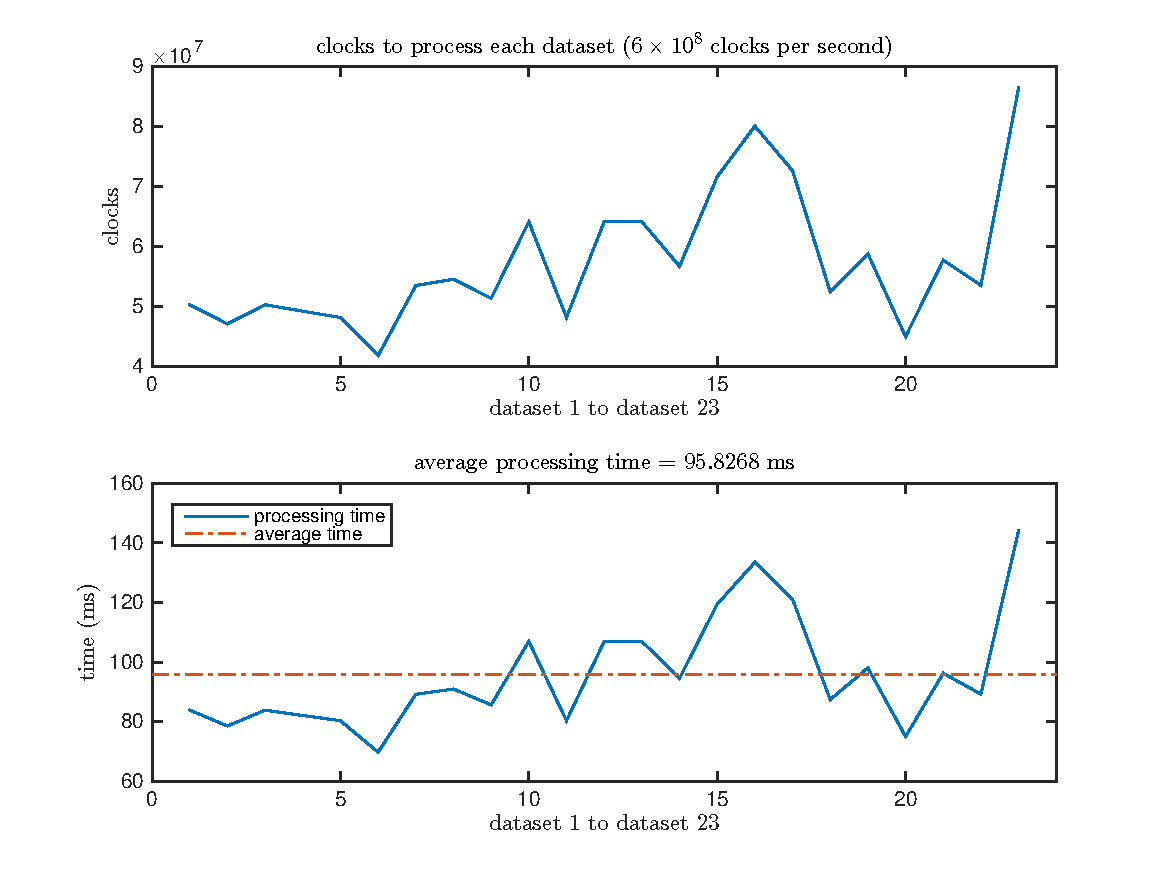
\includegraphics[width=3in, trim={0 0.6cm 0 0.6cm}, clip]{ang/processing_time}
\end{figure}
\end{frame}

%--------------------------------------------
%--------------------------------------------

\begin{frame}
\begin{itemize}
\item Probabilities of 27 words computed by MATLAB (\textcolor{navy_matlab}{navy circle $\circ$})
\item Probabilities of 27 words computed by DSP (\textcolor{orange_matlab}{orange cross $\times$})
\item Dataset 1 has the largest relative error among 23 datasets.
\end{itemize}

\begin{figure}[H]
\centering
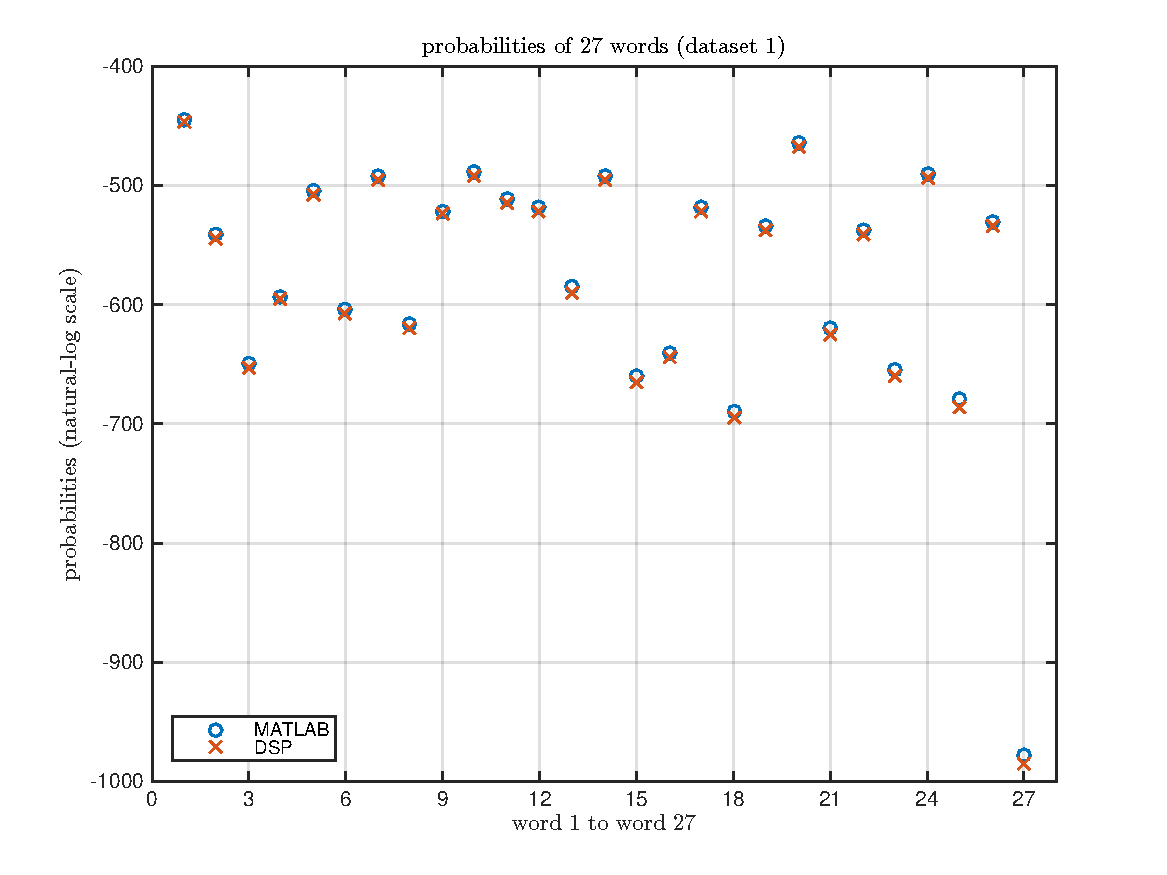
\includegraphics[width=3in, trim={0 0.6cm 0 0.6cm}, clip]{ang/word_probabilities}
\end{figure}
\end{frame}

%----------------------------------------------------------------------------------------
%	Subsection
%----------------------------------------------------------------------------------------

\begin{frame}
\frametitle{Final system implemented on DSP board}
\begin{itemize}
	\item Adaptive noise cancellation based on Least Mean Square Algorithm
	\item Real-time recognition of spoken words
	\item Result indication via a five-LED array
		\begin{itemize}
		\item \LED\offLED\offLED\offLED\offLED\onLED $\longrightarrow$ $(00001)_2 = 1$ $\longrightarrow$ word \textit{one}
		\item \LED\offLED\onLED\onLED\onLED\onLED $\longrightarrow$ $(01111)_2 = 15$ $\longrightarrow$ word \textit{fifteen}
		\item \LED\onLED\offLED\onLED\offLED\onLED $\longrightarrow$ $(10101)_2 = 21$ $\longrightarrow$ word \textit{zero}
		\item \LED\offLED\offLED\offLED\offLED\offLED $\longrightarrow$ $(00000)_2 = 0$ $\longrightarrow$ error
		\end{itemize}
	\item Wireless communication (WIFI)
	\item YouTube controller
		\begin{itemize}
		\item A Python program receives command and controls YouTube on PC.
		\end{itemize}
\end{itemize}
\end{frame}

%----------------------------------------------------------------------------------------
%	Subsection
%----------------------------------------------------------------------------------------

\begin{frame}
\frametitle{Utilization in Home Automation}
\begin{itemize}
	\item Arduino\textsuperscript{\textregistered} board as an intermediate
		\begin{itemize}
		\item the open-source ecosystem of abundant resources
		\item WIFI module $\longrightarrow$ wireless communication
		\item infrared emitter $\longrightarrow$ remote control of TV
		\item relay $\longrightarrow$ AC light switch
		\end{itemize}
\end{itemize}

\begin{figure}[H]
\centering
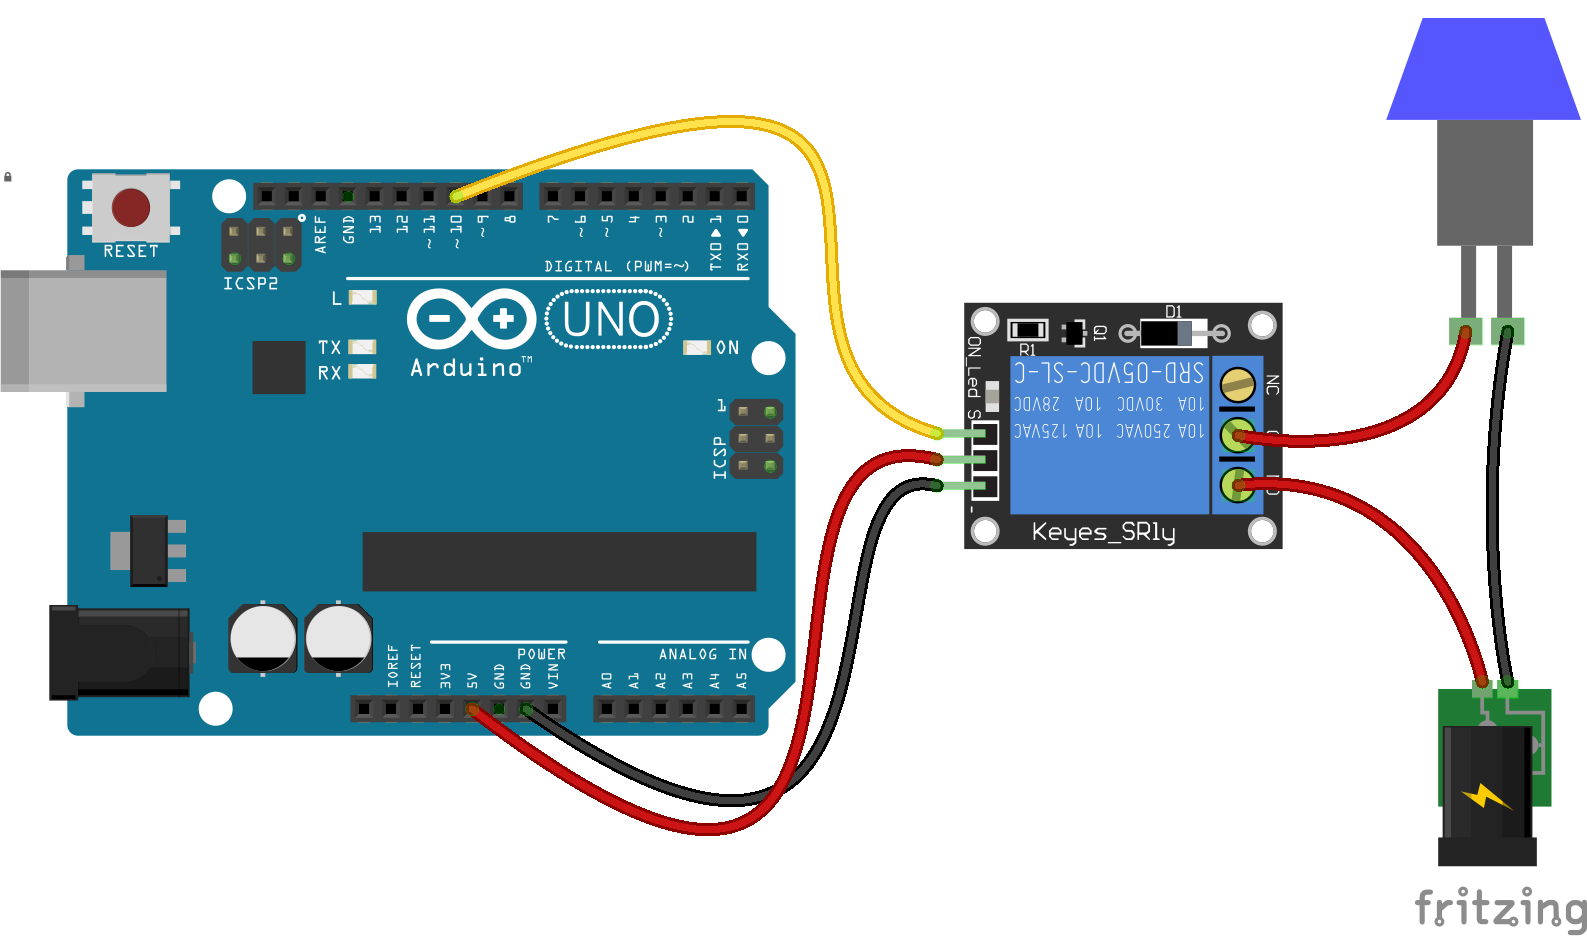
\includegraphics[width=0.5\textwidth]{ang/relay-arduino}
\caption{Control AC Light using Arduino with Relay Module \cite{relay-arduino}}
\end{figure}
\end{frame}
